\vspace{\baselineskip}
\begin{minipage}[t]{0.59\textwidth}
	\section{VHDL}
	Die vollst"andige Beschreibung des Designs (Grundstruktur) besteht aus:
	\begin{description}
	\setlength{\itemsep}{0pt}
  	\setlength{\parskip}{0pt}
  	\setlength{\parsep}{0pt}
		\item [library:] Bibliothekenbeschreibung
		\item [entity:] Schnittstellenbeschreibung
		\item [architecture:] Architekturbeschreibung
	\end{description}
	\subsection{Key Concepts}
	\begin{tabular}{ll}
		Key Concept I: & Schaltungshierarchie und Verbindung von Sub-Bl"ocken\\
		& (hierarchy and connectivity).\\
		Key Concept II: & Nebenl"aufige (concurrent) Prozesse und Prozess-\\
		& Interaktion.\\
		Key Concept III: & Modellierung des elektrischen Verhaltens von Signalen.\\
		Key Concept IV: & Event-Based time: Simulationsmodell, das auf Events\\
		& und nicht auf kontinuierlicher Zeit beruht.\\
		Key Concept V: & Parametrisierung von Modellen.
	\end{tabular}
\end{minipage}
\begin{minipage}[t]{0.3\textwidth}
\subsection{Identifier}
		\begin{itemize}
			\setlength{\itemsep}{0pt}
  			\setlength{\parskip}{0pt}
  			\setlength{\parsep}{0pt}
				\item Start mit Buchstabe
				\item \_ nicht am Ende oder doppelt
				\item case insensitive
				\item Eigene Identifier $\rightarrow$ GROSSBUCHSTABEN
				\item Library Identifier $\rightarrow$ kleinbuchstaben
		\end{itemize}
		\vfill\null
\end{minipage}
	
\begin{minipage}[t]{0.59\textwidth}
	\subsection{Bibliotheken (library)}
	\begin{tabular}{ll}
		work & Default-Bibliothek des Benutzers \\
		std & standard (Vordefinierte Datentypen und Funktionen),\\
		& textio (Text -  Filehandling)\\
		work und std &m"ussen nicht deklariert werden (automatisch eingebunden)\\
		ieee & std\_logic\_1164: Datentypen f"ur mehrwertiges Logiksystem\\
		& numeric\_std: Mathe-Bibliothek f"ur std\_logic
	\end{tabular}
	Mit \textbf{use} wird Bibliotheksinhalt im ganzen VHDL Modul sichtbar.
\end{minipage}
\hfill
\begin{minipage}[t]{0.3\textwidth}
	\lstinputlisting[language=VHDL,tabsize=2]{code/header.vhd}
\end{minipage}

\subsection{Schnittstellenbeschreibung (entity)}
	Die einzelnen Bl"ocke einer VHDL-Beschreibung kommunizieren "uber ihre 
	Schnittstellen miteinander. Die Kommunikationskan"ale nach aussen sind sogenannte Ports. F"ur diese werden in der Schnittstellenbeschreibung Name, Signalflussrichtung und Datentyp festgelegt. Mit der Signalflussrichtung werden Eing"ange, Ausg"ange und bidirektionale Ports unterschieden.
	\vspace{-\baselineskip}
	\begin{multicols}{2}
		\lstinputlisting[language=vhdl,tabsize=2]{code/entity.vhd}
		\lstinputlisting[language=vhdl,tabsize=2]{code/entity_bsp.vhd}
	\end{multicols}
\begin{multicols}{2}
\subsubsection{Signalflussrichtungen (mode)}
	\begin{tabular}{ll}
		in: & Eingangssignal. Darf nur rechts stehen.\\
		out: & Ausgangssignal. Darf nur links stehen.\\
		buffer: & Ausgangssignal. Darf auch rechts stehen\\
		&  $\rightarrow$ \textbf{problematisch}\\
		inout: & Bidirektionales Signal, \\
		& in Verbindung mit Typ std\_logic.\\
	\end{tabular}
\vfill\null
\subsubsection{Signaltypen (type)}
	\begin{tabular}{ll}
		boolean & Werte: true, false\\
		bit & Werte: '0','1'\\
		bit\_vector: & eindimensionaler Array von bits\\
		integer & interne Darstellung mit 32bit,\\
		& Range-Einschr"ankung n"otig!\\
		std\_logic(\_vector) & wie bit(\_vector), aber f"ur einen Treiber\\
		std\_ulogic(\_vector) & '', aber für mehrwertige Logik\\
	\end{tabular}
\end{multicols}
	
\begin{multicols}{2}	
	\subsection{Architekturbeschreibung (architecture)}
	Die Architektur legt die Funktion eines Blocks fest. Dabei kann eine entity mehrere architectures besitzen. Für die Simulation und Synthese müssen aber alle nicht verwendeten Architekturen auskommentiert werden.
	\lstinputlisting[language=VHDL,tabsize=2]{code/architecture.vhd}
	\vfill\null
	\columnbreak
	\subsubsection{Signaldeklaration}
	 Hier werden die Signale, die Innerhalb der Architektur verwendet werden, deklariert.
	\lstinputlisting[language=vhdl,tabsize=2]{code/signal.vhd}
	\subsubsection{Komponentendeklaration}
		Mit Hilfe des Schl"usselwortes \textbf{component} erfolgt die Deklaration von Komponenten, "ahnlich wie einer \textbf{entity}.\\
		\lstinputlisting[language=vhdl,tabsize=2]{code/component.vhd}
\end{multicols}%
\vspace{-2\baselineskip}
\begin{multicols}{2}
Häufige architecture\_names:
\begin{itemize}
	\setlength\itemsep{-0.5em}
	\item behavioral (Verhaltensbeschreibung einer Designeinheit)
	\item RTL (Register Transfer Level)
	\item Dataflow (Netzliste mit booleschen Operatoren)
	\item Structural (Strukturbeschreibung einer Designeinheit)
	\item Tb (Test-Bench)
\end{itemize}
\end{multicols}

\vspace{-\baselineskip}
\begin{multicols}{2}
	\subsubsection{Anweisungsteil}
	Im Anweisungsteil wird das Verhalten beschrieben. Dabei werden verschiedene Modellierungsstile unterschieden.
	\paragraph{Strukturmodell (Instanzierung)}
	Die Ein- und Ausgänge von Komponenten, die in einer Bibliothek abgelegt sind werden durch lokale Signale miteinander verbunden $\rightarrow$ Es entsteht eine Netzliste. 
	\lstinputlisting[language=vhdl,tabsize=2]{code/instanzierung.vhd}
	%\columnbreak
	\paragraph{Datenflussmodell}
	Es werden logische Grundfunktionen verwendet.
	Logikoperatoren f"ur bit, bit\_vector, boolean: \textbf{not, and, or, nand, nor, xor, xnor}. Wenn auf bit\_vector angewendet, dann muss Bitbreite von beiden Operanden gleich sein.
	\lstinputlisting[language=vhdl,tabsize=2]{code/datenfluss.vhd}
	\paragraph{Verhaltensmodell} ($\rightarrow$ H"aufigster Modellierungsstil.) 
	Die Modellierung findet durch Sprachelemente "ahnlich wie in einer prozeduralen Programmiersprache statt. Dabei werden abgeschlossene Hardware-Bl"ocke durch Prozesse 
	abgebildet.
\end{multicols}
			
\begin{multicols}{2}
	\subsection{Signalzuweisung}
	Alle Signalzuweisungen und alle Prozesse laufen parallel zueinander. Signalzuweisungen sind immer aktiv. Signale k"onnen auf verschiedene Arten zugewiesen werden:
	\lstinputlisting[language=vhdl,tabsize=2]{code/signalzuweisung.vhd}
%	\vfill\null
%	\columnbreak
	\subsubsection{Aggregat}
	Ein Aggregat ist ein Klammerausdruck, der mehrere Einzelelemente zu einem Vektor zusammenfasst.
		\lstinputlisting[language=vhdl,tabsize=2]{code/aggregat.vhd}
\end{multicols}
	
\begin{multicols}{2}
	\subsection{Prozesse}
	\begin{itemize}
	\setlength{\itemsep}{1pt}
	\setlength{\parskip}{0pt}
	\setlength{\parsep}{0pt}
		\item Prozesse werden durch Änderungen der Signale in der Sensitivitätsliste aktiviert und ausgeführt.
		\item Prozesse verhalten sich gegen aussen nebenl"aufig, innerhalb werden Anweisungen sequentiell abgearbeitet.
		\item \textbf{Selektive und bedingte Signalzuweisungen sind verboten.}
		\item Unbedingte Signalzuweisungen sind erlaubt. 
		\item \textbf{Aktualisierung aller Signale geschieht immer erst am Prozessende!}
		\item Zuweisen eines \textbf{Default-Wertes} an alle Ausgangssignale vor der ersten if-Anweisung zur Vermeidung von Latches.
		\item Hint: Damit Code übersichtlich und verständlich bleibt, sollte \textbf{nicht zu viel Funktionalität} in einen einzigen Prozess verpackt werden.
		\item Alle Signale, die auf der rechten Seite einer Signalzuweisung stehen, gehören in Sensitivitätsliste.
		\item Ohne Sensitivitätsliste nur in Simulation erlaubt.
	\end{itemize}
	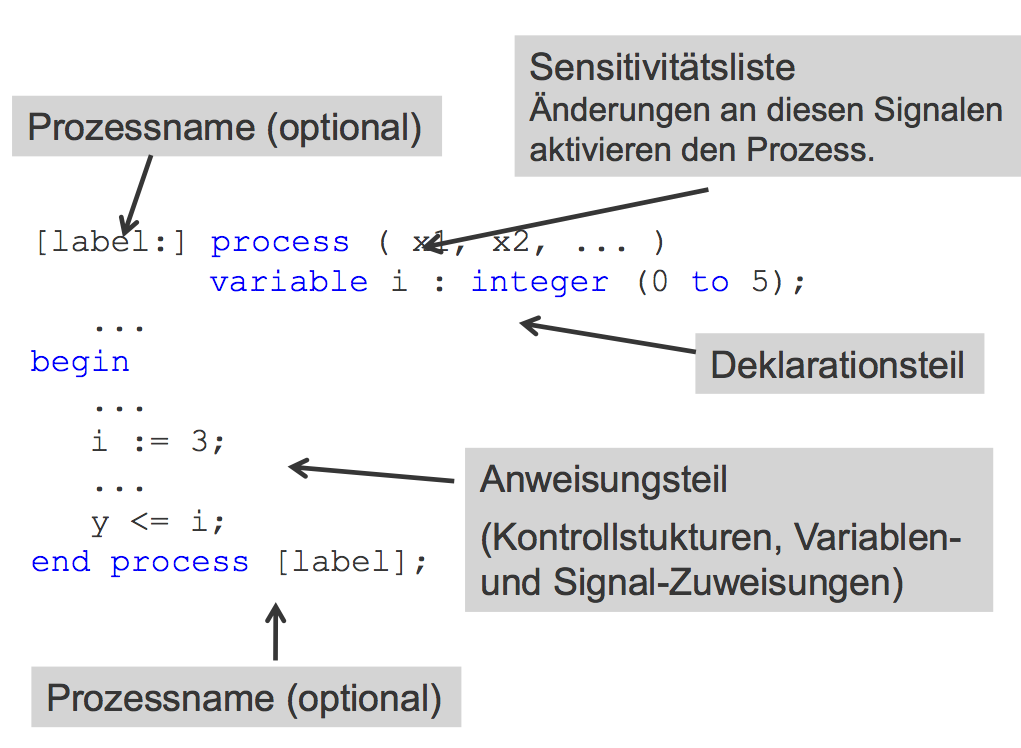
\includegraphics[width=0.4\textwidth]{images/syntaxprozess}
	\vfill\null
	\columnbreak
	\subsubsection{Variablen}			
	\begin{itemize}
		\setlength{\itemsep}{1pt}
		\setlength{\parskip}{0pt}
		\setlength{\parsep}{0pt}
		\item Variablen werden im Deklarationsteil des Prozesses deklariert und sind nur in diesem Prozess sichtbar.
		\item Zugewiesener Wert kann sofort abgefragt werden
		\item Wertzuweisung durch Operator \textbf{:=} (nicht $<$=)
		\item Vor Verwendung einen aktuellen Wert (evtl. Default-Wert) zuweisen, sonst entsteht ein Latch.
	\end{itemize}
	\vspace{-\baselineskip}
	\lstinputlisting[language=vhdl,tabsize=2]{code/variable.vhd}
		
	\subsubsection{Signalzuweisung durch Prozesse}
	\lstinputlisting[language=vhdl,tabsize=2]{code/kontrollstruktur.vhd}
\end{multicols}

\newpage

\begin{multicols}{2}
	\subsection{Sequentielle Systeme}
	\subsubsection{Flankenerfassung}
		\lstinputlisting[language=vhdl,tabsize=2]{code/flanke.vhd}
	\subsubsection{Zustandscodierung}
	\begin{itemize}
	\itemsep0em
		\item Die Deklaration der Zustandscodierung erfolgt im Deklarationsteil der Architektur.
		\item Bei expliziter Zustandscodierung muss diese in der IDE auf $"$User$"$ umgestellt werden.
	\end{itemize}
	\lstinputlisting[language=vhdl,tabsize=2]{code/zustandscode.vhd}
	\vfill\null
	\columnbreak
	\subsubsection{FSM in 3-Prozess Struktur}
	Die Zustandsmaschine wird in 3 Prozesse aufgeteilt. Diese Prozesse werden ganz einfach einzeln im Anwendungsteil der Architektur implementiert und arbeiten jeweils nebenl"aufig.
	\begin{center}
		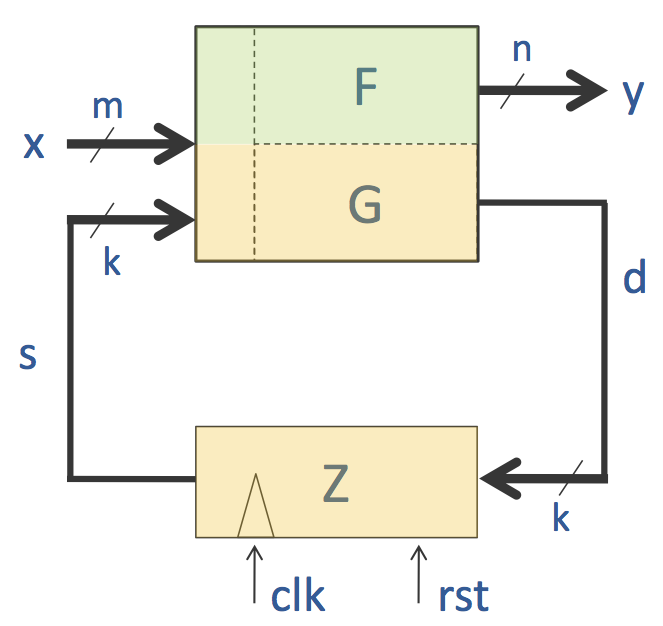
\includegraphics[width=0.13\textwidth]{images/fsmprocesslogic}
	\end{center}
	\begin{itemize}
		\setlength\itemsep{-0.5em}
		\item Prozess F = Output\_Logic (reine Logik)
		\item Prozess G = Next\_State\_Logic (reine Logik)
		\item Prozess Z = State\_Register (Logik mit Speicher)
	\end{itemize}

	\paragraph{Output\_Logic}
	Dieser kombinatorische Teil ist abhängig von der Struktur der FSM. Häufig Case für State und If / elsif für Inputs (Mealy).
	\lstinputlisting[language=vhdl,tabsize=2]{code/outputlogic.vhd}
\end{multicols}

\begin{multicols}{2}
	\paragraph{Next\_State\_Logic} 
	Dieser kombinatorische Teil ist nicht abh"angig von der Struktur der FSM.
	\lstinputlisting[language=vhdl,tabsize=2]{code/nextstatelogic.vhd}
	\vfill\null
	\columnbreak
	\paragraph{State\_Register}  
	Dieser kombinatorische Teil ist nicht abh"angig von der Struktur der 
	FSM und sieht bei allen (fast) FSM immer gleich aus.
	\lstinputlisting[language=vhdl,tabsize=2]{code/stateregister.vhd}
\end{multicols}

\begin{multicols}{2}
	\subsection{IEEE 1164 Logiksystem}
	Die ieee.std\_logic\_1164 Library enthält die std\_logic, sowie std\_ulogic Datentypen. 9-wertige Logik:
	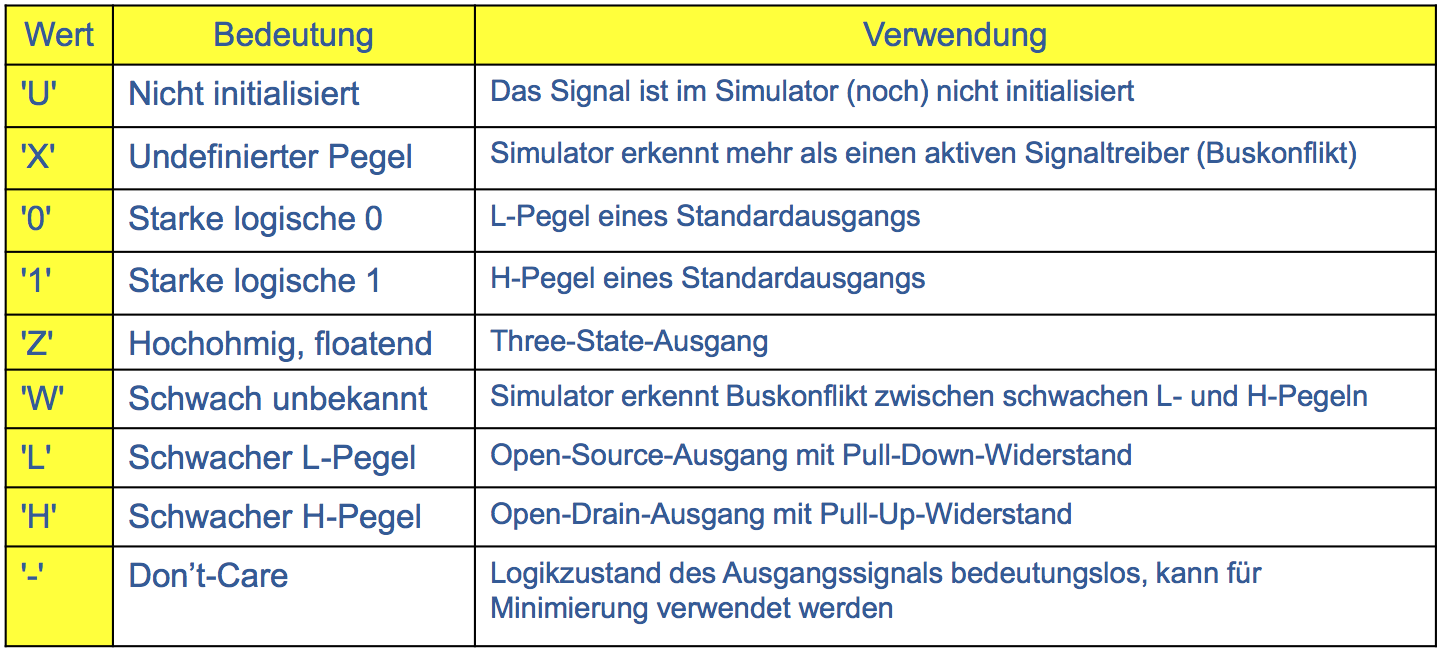
\includegraphics[width=0.45\textwidth]{images/ieee1164logicsystem}
	
	\vfill\null
	\columnbreak
	\subsubsection{TriStateLogic}
	\lstinputlisting[language=vhdl,tabsize=2]{code/buscontrol.vhd}
\end{multicols}

\begin{multicols}{2}
	\subsection{Type-Casting/-Conversion}
	\begin{center}
		\includegraphics[width=0.37\textwidth]{images/typeConversions}
	\end{center}
	\vfill\null
	\columnbreak
	\subsection{Arithmetik}
	\begin{minipage}{0.4\linewidth}
		Durch zus"atzliches Einbinden der ieee.numeric\_std neben ieee.std\_logic\_1164 stehen signed und unsigned Datentypen auf Basis des std\_logic\_vector Datentyps, sowie arithmetische Operatoren und Vergleichsfunktionen zur Verf"ugung.
	\end{minipage}
	\begin{minipage}{0.55\linewidth}
		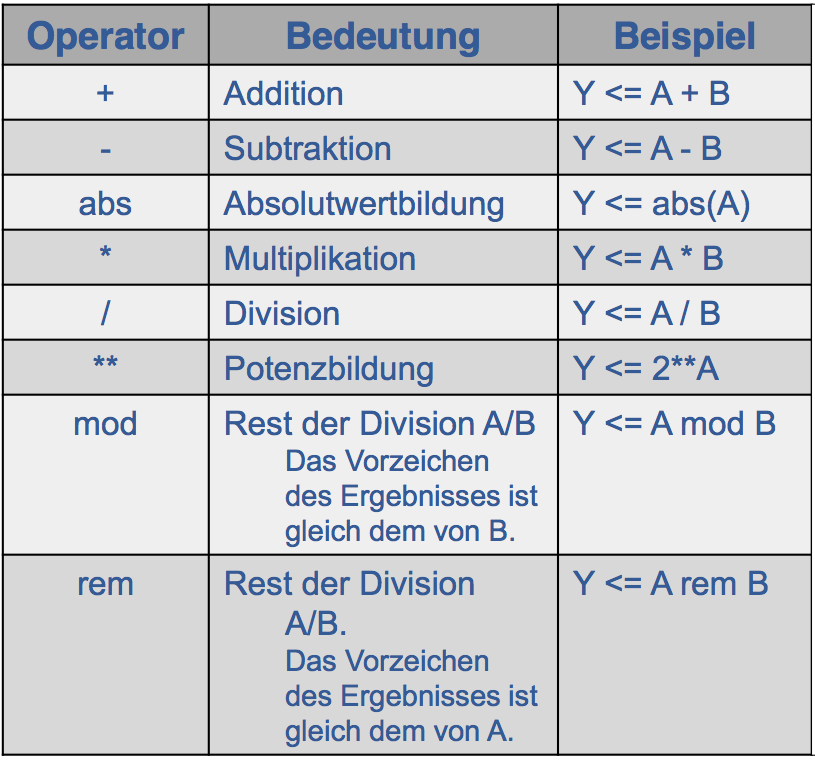
\includegraphics[width=\linewidth]{images/arithoperator}
	\end{minipage}
	% Bild 'Arithvergleich' ist aus Formatierungsgründen in nächstem Abschnitt eingefügt.
\end{multicols}
\vspace{-3\baselineskip}
\begin{multicols}{2}
\subsection{resize}
	Vektoren vom Typ unsigned und signed können auf gewünschte Länge gebracht werden.
	\lstinputlisting[language=vhdl, tabsize=2]{code/resize.vhd}
	\begin{center}
		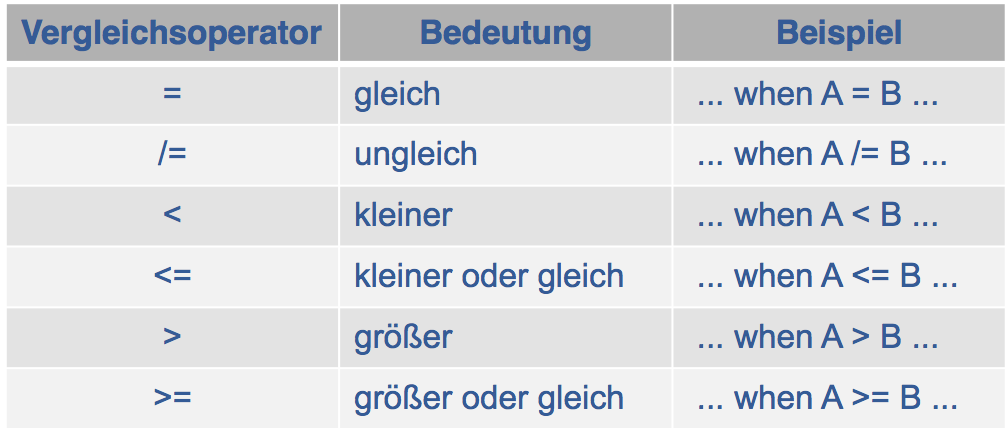
\includegraphics[width=0.4\textwidth]{images/arithvergleich}
	\end{center}
\end{multicols}
\vspace{-2\baselineskip}
\begin{multicols}{2}
	\subsection{Simulation}
	\subsubsection{Aufbau einer Test-Bench}
	Die Test-Bench soll wiederverwertbar sein, ist jedoch nicht synthesefähig. Arbeitet nach Delta-time-Prinzip. (Event queue definiert Events). Normales VHDL Modul bestehend aus:
	\vspace{-\topsep}
	\begin{itemize}
	\setlength\itemsep{-0.5em}
		\item library
		\item entity (i.d.R. ohne Ports nach aussen) $\rightarrow$ leer
		\item architecture
		\begin{itemize}
			\setlength\itemsep{-0.5em}
			\item Komponenten (DUT) Deklerationen
			\item ggf. Auswahl der DUT-Architektur
			\item (Timing-Informationen als Konstante (oder 
				Generic) deklarieren)
			\item Signale deklarieren (Benennung: $<$DUT\_SIG$>$\_tb)
			\item Instanzierung des DUT
			\item Prozess für Clock-Erzeugung
			\item Prozess für die Anwendung von Stimuli 
				(Stimulusgenerator)
			\item Prozess für das Erfassen der Systemantwort 
				(Response-Monitor)
		\end{itemize}
	\end{itemize}
\end{multicols}

\begin{multicols}{2}
	\subsubsection{Testbench}
	\lstinputlisting[language=vhdl,tabsize=2]{code/testbench.vhd}
\end{multicols}

%			\paragraph{DUT einbinden und konfigurieren (in Deklarationsteil)} DUT wird als Komponente ganz normal deklariert.
%				Sind mehrere Architekturen vorhanden, muss die zu stimulierende 	
%				Architektur ausgewählt werden:
%				\lstinputlisting[language=vhdl,tabsize=2]{code/configarchitecture.vhd}
%			\begin{multicols}{2}
%				\paragraph{Timing-Konstante} 
%					\lstinputlisting[language=vhdl,tabsize=2]{code/timeconstant.vhd}
%				\paragraph{Clock-Prozess}
%					\lstinputlisting[language=vhdl,tabsize=2]{code/clockprozess.vhd}
%				\paragraph{Stimulusgenerator} 
%					\lstinputlisting[language=vhdl,tabsize=2]{code/stimulusgenerator.vhd}
%			\end{multicols}	
\vspace{-\baselineskip}
\begin{minipage}{0.63\textwidth}
	\paragraph{Response-Monitor (inkl. Assert)}
		\lstinputlisting[language=vhdl,tabsize=2]{code/responsemonitor.vhd}
\end{minipage}
\hfill
\begin{minipage}{0.35\textwidth}
	\subsubsection{For-Loop} % Evt. als paragraph, wenn Platzmangel
	For-Loops finden Verwendung in der \colorbox{yellow}{Simulation}, oftmals in Verbindung mit wait-Statements und daher ohne Sensititvit"atsliste. Sie k"onnen aber auch synthetisiert werden, daf"ur muss der Range 
	endlich sein.
	\lstinputlisting[language=vhdl,tabsize=2]{code/forloop.vhd}
\end{minipage}
					
\begin{multicols}{2}
	\subsubsection{Verz"ogerungszeiten}  % Evt. als paragraph, wenn Platzmangel
	\begin{itemize}
		\itemsep0em
		\item $\Delta$-Time $\rightarrow$ funktioneller Zusammenhang 
			zwischen Ursache/Wirkung (automatisch)
		\item inertial delay (Tr"agheit) $\rightarrow$ Ausgang "andert erst, wenn Eingang l"anger konstant bleibt als mit \textbf{after} definiert (Nicht verwenden f"ur Verz"ogerungszeit)
%		\vfill\null
%		\columnbreak
		\lstinputlisting[language=vhdl,tabsize=2]
				{code/inertial.vhd}
		\item transport delay $\rightarrow$ Ausgang "andert nach Eingans"anderung mit \textbf{after} definierter Zeit 
			\lstinputlisting[language=vhdl,tabsize=2]{code/transport.vhd}
		\vfill\null
		\columnbreak	
		\subsection{Generic}
		$\rightarrow$ Re-Use! So kann VHDL Parameter an ein Modell 
		"ubergeben.\ Dabei wird der Parameter wie eine Konstante im Anweisungsteil verwendet.\\
		Daf"ur muss in jeder Schnittstellenbeschreibung der Generic-Block eingbaut werden:
		\lstinputlisting[language=vhdl,tabsize=2]{code/generic.vhd}
		Bei der Instanzierung wird mit generic map der Parameter-Wert gesetzt.\\
		Der generic-Parameter wird zur Compile-Zeit fixiert.
		\vfill\null
	\end{itemize}
\end{multicols}
	
\begin{multicols}{2}


	\subsubsection{Beispiel für Implementation}
	Die Implementation geschieht wie auch bei den anderen 
	Komponenten meistens in einer separaten Datei, einfach enth"alt hier die entity noch ein generic.
	\lstinputlisting[language=vhdl,tabsize=2]{code/generic_dekleration.vhd}
	\vfill\null
	\columnbreak
	\subsubsection{Beispiel für Instanzierung}
	Auch hier wird wie gewohnt zuerst die Komponente deklariert und 
	anschliessend im Anwendungsteil instanziert.
	\lstinputlisting[language=vhdl,tabsize=2]{code/generic_instanzierung.vhd}
\end{multicols}